\documentclass[11pt,numbers=noenddot]{scrreprt}
\KOMAoptions{paper=a4}
\KOMAoptions{twoside=false}
%\KOMAoptions{footinclude=true}
%\KOMAoptions{headinclude=true}
\KOMAoptions{cleardoublepage=current}
%\KOMAoptions{draft=true}

\usepackage[ngerman]{babel}
\usepackage[T1]{fontenc}
\usepackage[ansinew]{inputenc}

%\usepackage[T1]{fontenc}
%\usepackage[utf8x]{inputenc}
%\usepackage[utf8]{inputenc}
%\DeclareUnicodeCharacter{A4C3}{ä}
%\DeclareUnicodeCharacter{C3B6}{ö}
%\DeclareUnicodeCharacter{C3BC}{ü}
%\DeclareUnicodeCharacter{C384}{ä}
%\DeclareUnicodeCharacter{C396}{ö}
%\DeclareUnicodeCharacter{C39C}{ü}

%\usepackage{ngerman}
\usepackage{enumerate}
%\usepackage{eurosym}
%\usepackage{lastpage}	% nötig, wenn man die Gesamtanzahl der Seite verwenden will - \pageref{LastPage}
\usepackage[automark]{scrpage2}
%\usepackage{fancybox}	% nötig, wenn man anstatt \fbox \ovalbox haben möchte

\usepackage{wrapfig}
\usepackage{subfigure}

% -- colors
\usepackage{color}
\definecolor{Skyblue}{rgb}{0.204, 0.396, 0.643} % #3465a4
\definecolor{LightSkyblue}{rgb}{0.447, 0.624, 0.818}	% #729fcf
\definecolor{DarkSkyblue}{rgb}{0.125, 0.290, 0.529}	% # 204a87

%-----------------------------------------------------------------------------%
% farbige Überschriften
%-----------------------------------------------------------------------------% 
\addtokomafont{part}{\normalfont\Huge\bfseries\sffamily\textcolor{Skyblue}}
\addtokomafont{partnumber}{\normalfont\Huge\bfseries\sffamily\textcolor{Skyblue}}
\addtokomafont{chapter}{\textcolor{Skyblue}}
\addtokomafont{section}{\textcolor{Skyblue}}
\addtokomafont{subsection}{\textcolor{Skyblue}}
\addtokomafont{subsubsection}{\textcolor{Skyblue}}
\addtokomafont{paragraph}{\textcolor{Skyblue}}
\addtokomafont{subparagraph}{\textcolor{Skyblue}}

\usepackage{hyperref}
\hypersetup{
%	pdftex, 
	colorlinks=true, 
	linkcolor=DarkSkyblue, 
	citecolor=LightSkyblue, 
%	filecolor=blue, 
	urlcolor=Skyblue, 
	pdftitle=Ipponboard Handbuch, 
%	pdfauthor=Florian Mücke, 
%	pdfsubject=, 
%	pdfkeywords=
}
%\usepackage[pdftex]{graphicx}
\usepackage{graphicx}

%\usepackage[T1]{fontenc}
%\usepackage{avant}
%\renewcommand*\familydefault{\sfdefault} 

\usepackage{fontspec} 

%\usepackage{fontspec} 
%\fontspec[ 
%	BoldFont=MyriadPro-Bold.otf, 
%	ItalicFont=MyriadPro-It.otf,
%	BoldItalicFont=MyriadPro-BoldIt.otf]
%{MyriadPro-Regular.otf}
%\setmainfont{Myriad Pro} %PT Sans
%\setsansfont{Myriad Pro}

\fontspec[ 
	BoldFont=PT_Sans-Bold.ttf, 
	ItalicFont=PT_Sans-Italic.ttf,
	BoldItalicFont=PT_Sans-BoldItalic.ttf]
{PT_Sans-Regular.ttf}
\setmainfont{PT Sans}
\setsansfont{PT Sans Caption}
\defaultfontfeatures{Mapping=tex-text}

%\fontspec[ 
%	BoldFont=ArnoPro-Bold.otf, 
%	ItalicFont=ArnoPro-Italic.otf,
%	BoldItalicFont=ArnoPro-BoldItalic.otf]
%{ArnoPro-Regular.otf}
%\setmainfont{}
%\setsansfont{ACaslonPro-Semibold.otf}
%\defaultfontfeatures{Mapping=tex-text}

%\fontspec[ 
%	BoldFont=Vollkorn-Bold.ttf, 
%	ItalicFont=Vollkorn-Italic.ttf,
%	BoldItalicFont=Vollkorn-BoldItalic.ttf]
%{Vollkorn-Regular.ttf}


\newcommand*{\IB}{\begingroup{\fontspec{Cuprum}\selectfont\textsc{Ipponboard}} \endgroup}
\newcommand*{\IBVersion}{0.4.2}
\newcommand*{\mybox}[1]{ \vskip 1.0em \noindent\fbox{\parbox[t]{\linewidth}{\itshape#1}} \vskip 0.5em }


% Outline numbering
%\setcounter{secnumdepth}{4}
%\renewcommand\thesection{\arabic{section}}
%\renewcommand\thesubsection{\arabic{section}.\arabic{subsection}}
%\renewcommand\thesubsubsection{\arabic{section}.\arabic{subsection}.\arabic{subsubsection}}
%\renewcommand\theparagraph{\arabic{section}.\arabic{subsection}.\arabic{subsubsection}.\arabic{paragraph}}

% Page layout (geometry)
%\setlength\voffset{-1in}
%\setlength\hoffset{-1in}
%\setlength\topmargin{1.499cm}
%\setlength\oddsidemargin{1.499cm}
%\setlength\textheight{15.009cm}
%\setlength\textwidth{26.702cm}
%\setlength\footskip{1.497cm}
%\setlength\headheight{0.998cm}
%\setlength\headsep{0.499cm}

% Footnote rule
%\setlength{\skip\footins}{0.119cm}
%\renewcommand\footnoterule{\vspace*{-0.018cm}\setlength\leftskip{0pt}\setlength\rightskip{0pt plus 1fil}\noindent\textcolor{black}{\rule{0.25\columnwidth}{0.018cm}}\vspace*{0.101cm}}

% Pages styles
\makeatletter
\newcommand\ps@Standard{
  \renewcommand\@oddhead{ \hfill {\IB} v\IBVersion}
  \renewcommand\@evenhead{\@oddhead}
  \renewcommand\@oddfoot{{\small \textcopyright 2010 Florian Mücke, Stand: \today}\hfill \thepage{}}
  \renewcommand\@evenfoot{\@oddfoot}
  %\renewcommand\thepage{\arabic{page}}
}
\makeatother

\pagestyle{Standard}
\renewcommand*{\chapterpagestyle}{Standard}

% footnotes configuration
\makeatletter
\renewcommand\thefootnote{\arabic{footnote}}
\makeatother

\title{{\IB} Anzeigesystem}
\subtitle{Version \IBVersion}
%\author{Florian Mücke}
\date{\today}

%--------------------------------%
%% ->->-> BEGIN DOCUMENT <-<-<- %%
%--------------------------------%
\begin{document}
\maketitle

\thispagestyle{empty}

\vspace*{\fill}

{\centering\bfseries\itshape\LARGE
Dieses Dokument befindet sich noch im Aufbau.\\
Der vorliegende Inhalt kann und wird sich ändern.\\
Es besteht kein Anspruch auf Vollständigkeit! \par}

\vspace*{\fill}

\begin{center}
{%\parindent 0pt
Copyright \textcopyright 2010 Florian Mücke \\
Webseite: \url{http://flo.mueckeimnetz.de/ipponboard} \\
Support, Bugtracking: \url{http://ipponboard.origo.ethz.ch/}}
\end{center}


%\setcounter{tocdepth}{10}
\renewcommand\contentsname{Inhalt}
\tableofcontents

\chapter{Version}

\section{Lizenz}
{\parindent 0pt \IB Copyright \textcopyright 2010 Florian Mücke.\\

Creative Commons Lizenz: Namensnennung-Keine Bearbeitung 3.0 Unported\\
\url{http://creativecommons.org/licenses/by-nd/3.0/deed.de}\\

Lizenzen für besondere Dateien sind folgende:
\begin{itemize}
	\item Qt (\texttt{QtCore4.dll}, \texttt{QtGui4.dll}): LGPL
	\item Microsoft Visual C++ CRT (\texttt{msvcm*.dll}, \texttt{msvcp*.dll}, \texttt{msvcr*.dll}):\\
	Visual Studio 2008/2010 License
	\item Sounddateien: Public Domain
\end{itemize}

Verwendete Bibliotheken:
\begin{itemize}
	\item Qt framework
	\item Boost C++ libraries (\href{http://www.boost.org/}{www.boost.org})
\end{itemize}

Weitere Informationen findet ihr in der \texttt{Lizenz.txt}-Datei.

\mybox{\textbf{Hinweis:} {\IB} darf frei auf beliebig vielen Rechnern innerhalb des Testzeitraums verwendet und das Programm in unveränderter Form auch unentgeltlich an dritte weitergeben werden.}
}

\newpage
\section{(System-)Voraussetzungen}
Um das \IB Anzeigesystem nutzen zu können gelten folgende Hard- und Softwareanforderungen:
\begin{itemize}
	\item Computer mit mind. Windows\texttrademark XP, der über einen zweiten Monitoranschluss verfügt (vorzugsweise ein Laptop)
	\item Fernseher oder großen Computerbildschirm für die Anzeige
	\item Verbindungskabel Computer $\leftrightarrow$ Zweitbildschirm
	\item USB-Gamepad zur Steuerung der Anzeige (z.B.\,Saitek P380)
	\item optional: Lautsprecher für das Mattensignal
\end{itemize}

\newpage
\section{Kontakt}
\paragraph{Eure Meinung zählt!}
Wir finden zwar, dass das \IB Anzeigesystem schon ziemlich toll ist, trotzdem ist es sicher nicht fehlerlos und an der einen oder anderen Ecke bestimmt auch verbesserbar. \textit{Bitte helft mit \IB zu verbessern!}

\begin{itemize}
	\item[$\Rightarrow$] bringt eure Ideen und Vorschläge ein
	\item[$\Rightarrow$] probiert es in eurem Verein aus
	\item[$\Rightarrow$] sagt euren Freunden Bescheid
	\item[$\Rightarrow$] informiert uns über Fehler und Probleme mit der Bedienung
\end{itemize}
Wir haben speziell zu diesem Zweck ein Umfrage-Formular im Web bereitgestellt. Dieses könnt ihr über folgende Adresse erreichen:
\begin{quote}
	\url{http://flo.mueckeimnetz.de/ipponboard/survay_de/}
\end{quote}
{\parindent 0pt\textit{Bitte macht von diesen Möglichkeiten Gebrauch!}}

\paragraph{Aktuelle Version}
Bitte nutzen Sie stets die aktuellste Version. Sobald es eine neuere Version gibt, wird diese im Internet bereitgestellt. Sie kann auf den Projektseiten heruntergeladen werden.

\paragraph{Kontakt}
Fragen oder Verbesserungsvorschläge für das \IB Anzeigesystem können an die folgenden Stellen gerichtet werden:
\begin{itemize}
	\item deutsche Projektseite des Autors:\\\url{http://flo.mueckeimnetz.de/ipponboard}
	\item englische Projektseite (Bugtracking, Download, News, ...):\\\url{http://ipponboard.origo.ethz.ch/}
	\item E-Mail: \url{mailto:ipponboard@mueckeimnetz.de}
\end{itemize}

\newpage
\section{Danke}
Mein besonderer Dank gilt folgenden Leuten:
\begin{itemize}
	\item Heini Schäfer  für die Idee, den Ansporn, die Kritik und das Know-How
	\item Meiner Frau Anja für ihre Geduld
	\item Christophe Henry für MSM Bibliothek (jetzt: boost msm)
	\item Nokia/Trolltech für die Qt Bibliothek
	\item ETH Zürich für Origo subversion project hosting
\end{itemize}

sowie folgenden Vereinen für Vertrauen und Feedback:
\begin{itemize}
	\item TSV Königsbrunn
	\item Post SV Telekom Augsburg
	\item TSV Peiting
	\item \dots
\end{itemize}



\chapter{Programmbeschreibung}
{\IB} ist ein fortschrittliches Anzeigesystem für die Kampfzeit und die Kampfpunkte, das speziell für den Judowettkampf entwickelt wurde. Bei der Entwicklung wird auf die folgenden Punkte besonderes Augenmerk gelegt:
\begin{itemize}
	\item ausgezeichnete Lesbarkeit
	\item einfache Bedienung
	\item unkomplizierter Einsatz
\end{itemize}

Das Programm wird prinzipiell von einem PC (Laptop) aus bedient und mit Maus oder Gamepad gesteuert. {\IB} verwaltet zwei Anzeigen, eine externe für die Kämpfer~/~Betreuer~/~Publikum und eine für die Zeitnehmer. Die Anzeige der Zeitnehmer ist dabei gespiegelt, damit sie den Kämpfern besser zugeordnet werden kann.

\section{Anzeige(n)}
Die Anzeige besteht im Wesentlichen aus fünf Bereichen:
\begin{itemize}
	\item \textit{Kampfzeit}: Diese befindet sich am unteren Rand der Anzeige. Ist der Kampf unterbrochen wird die Kampfzeit \textit{rot} dargestellt, ansonsten \textit{gelb}.
	\item \textit{Wertungen}: Die Wertungen sind auf der Seite des jeweiligen Kämpfers gruppiert und in der jeweiligen Farbkombination gehalten (Weiß auf Blau bzw. Schwarz auf Weiß). Die Strafen sind durch rote Punkte symbolisiert.
	\item \textit{Haltegriffzeit}
	\item \textit{Kampfinformationen} (Mattennummer, aktuelle Gewichtsklasse)
	\item \textit{Namen} der Kämpfer
\end{itemize}

\subsection[Primäre Anzeige]{Primäre Anzeige}

\begin{figure}
	\centering
		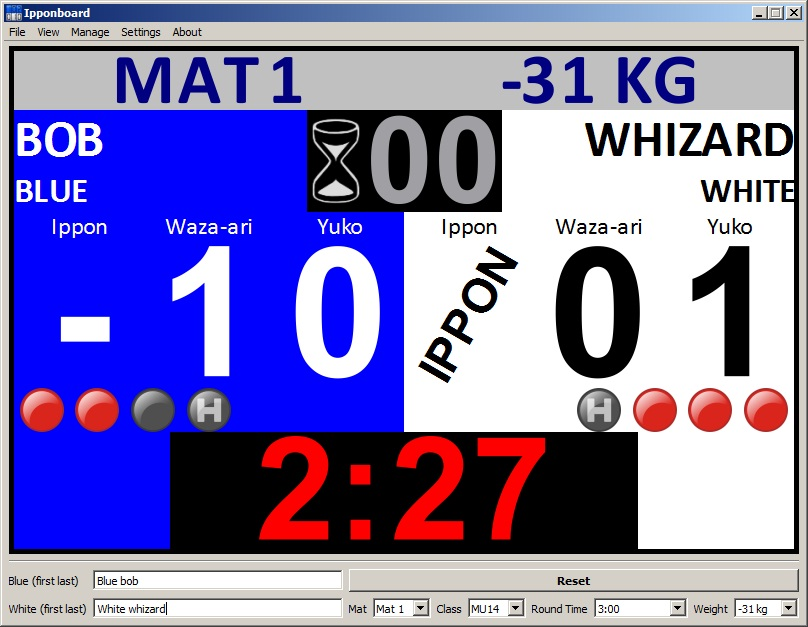
\includegraphics[width=0.8\textwidth]{images/primary_view.jpg}
	\caption{Primäre Anzeige}
	\label{fig:Primary_View}
\end{figure}

Die primäre Anzeige dient als zentrale Steuereinheit. Auf ihr sind alle Informationen verfügbar und einstellbar:
\begin{itemize}
	\item Kampf- und Haltegriffzeit starten/stoppen/(zurück-)setzen
	\item Kampf zurücksetzen
	\item Namen der Kämpfer ändern
	\item Wertungen setzen/zurücknehmen
	\item Kampfinformationen (Mattennummer, aktuelle Gewichtsklasse) ändern
\end{itemize}

\subsection{Sekundäre (externe) Anzeige}
Im Unterschied zur primären Anzeige werden auf der sekundären nur die für das Kampfgeschehen wesentlichen Details angezeigt:

\begin{itemize}
	\item nur die Wertungen bis Waza-ari (Ippon wird blinkend darübergelegt)
	\item nur die aktiven Strafen
	\item nur die aktive Haltegriffzeit
\end{itemize}

Eine weitere Einschränkung der sekundären Anzeige ist, dass sie bewusst nicht auf Eingaben mit der Maus reagiert.
Ob die zweite Anzeige beim Programmstart gleich angezeigt werden soll, oder auf welchem Bildschirm diese ausgegeben wird, lässt sich in den \textit{Programmeinstellungen} festlegen.

Wie der Rechner für den Zweischirmbetrieb ("`Dual-View"') konfiguriert werden muss, kann im Anhang: \textit{Computer 
für Zweischirmbetrieb vorbereiten} nachgelesen werden.

\mybox{\textbf{Tipp:} Aktivieren/Deaktivieren lässt sich die sekundäre Anzeige über den Hotkey \texttt{F2}.}


\section{Einstellungen}
\label{bkm:Programmeinstellungen}
Die Programmeinstellungen finden sind im Anwendungsmenü unter Einstellungen zu finden. Sie bieten Zugriff auf verschiedene \textit{allgemeine} Optionen zur Anpassung des Programms:
\begin{itemize}
	\item Sekundäre Anzeige konfigurieren
	\item Farben und Schriftart für den Info-Bereich ändern
	\item Farben für Kämpfer/Wertungen ändern
	%\item TODO:Schriftart für die Kampfzeit ändern
	\item Sounddatei für das Signal des Zeitnehmertisches auswählen
	%\item TODO: Standardeinstellungen wiederherstellen
\end{itemize}

Neben den allgemeinen Optionen lassen sich im Einstellungsmenü auch die Knöpfe des Gamepads neu belegen.

\begin{figure}[htp]
	\begin{center}
		\subfigure[Allgemeine Einstellungen]
			{\label{fig:Einstellungen_Allgemein}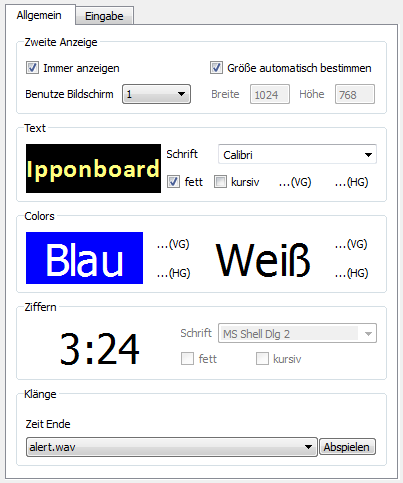
\includegraphics[scale=0.5]{images/Einstellungen_Allgemein.png}}
		\subfigure[Gamepad-Belegung ändern]
			{\label{fig:Gampad_Settings}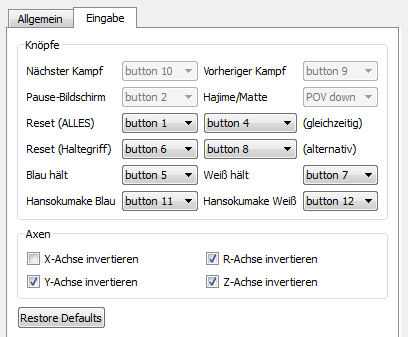
\includegraphics[scale=0.5]{images/Einstellungen_Eingabe.png}}
	\end{center}
	\caption{Einstellungsdialoge}
	\label{fig:Settings}
\end{figure}

\chapter{Steuerung}

{\IB} kann sowohl mit der Maus als auch mit dem Gamepad bedient werden\footnote{Die Steuerung über die Tastatur ist für spätere Versionen geplant.}. Damit das aktuell Kampfgeschehen möglichst unkompliziert und intuitiv wiedergegeben werden kann, lässt sich dieses vollständig mit einem der beiden Eingabegeräte
steuern.

Die Steuerung über die Maus mag zunächst einfacher erscheinen, da dieses Eingabegerät für die meisten vertraut ist und man die Anzeige intuitiv via Klicks ansprechen kann.

Unsere Erfahrungen haben jedoch gezeigt, dass mit dem Gamepad ein wesentlich entspannteres Bedienen als mit der Maus möglich ist. Daher möchten wir Ihnen die Steuerung mit dem Gamepad mit folgenden Gründen besonders ans Herz legen:

\paragraph*{Vorteile der Gamepad-Steuerung}
\begin{enumerate}
	\item \textit{Alles im Griff}

	Mit einem handelsüblichen USB-Gamepad kann auf alle wesentlichen Funktionen per Knopfdruck zugegriffen werden \-- egal ob Haltegriffanzeige, Kampfzeit, Wertungen oder Strafen. Dabei ist die linke Hand für den linken Kämpfer und die rechte für den rechten zuständig.

	\item \textit{Volle Konzentration auf das Kampfgeschehen}
	
	Der Blick muss nicht ständig zwischen Anzeigetafel und Matte hin- und herwechseln. Punkte können direkt eingegeben werden und es muss nicht ständig der Mauszeiger gesucht und erst umständlich auf das Wertungssymbol geschoben werden. Ein Knopfdruck und ein gelegentlicher flüchtiger Kontrollblick reichen völlig aus.
	
	\item \textit{Entspannt zurücklehnen}
	
	Das Beste daran: man kann sich ganz entspannt auf dem Stuhl zurücklehnen, anstatt konzentriert und angespannt vor der Maus zu sitzen.

	\item \textit{Coolness-Faktor}
	
	Für den Einsatz bei der Jugend sollte man den "`Coolness-Faktor"' nicht unterschätzen \-- so bedienen will wirklich jeder!
\end{enumerate}


\section{Gamepad-Steuerung}
\subsection{Aktionen}
\paragraph{Punkte vergeben und zurücknehmen}
{\begin{wrapfigure}{r}{0.3\textwidth}
  \centering
		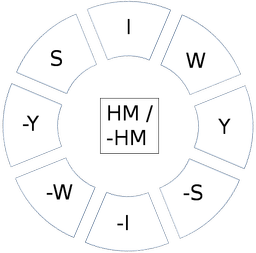
\includegraphics[width=0.3\textwidth]{images/Analogstick.png}
	\caption{Wertungsbelegung am Analogstick}
	\label{fig:Analogstick}
\end{wrapfigure}
Die Punkte werden über die beiden Analog-Sticks vergeben. Dabei entsprechen für den \emph{blauen} Kämpfer (linker Daumen!) folgende Richtungen den jeweiligen Punkten:
\begin{itemize}
	\item \emph{Ippon:} nach oben
	\item \emph{Ippon zurücknehmen}: nach unten
	\item \emph{Waza-ari:} rechts oben
	\item \emph{Waza-ari zurücknehmen:} links unten
	\item \emph{Yuko:} rechts
	\item \emph{Yuko zurücknehmen:} links
	\item \emph{Shido:} links oben
	\item \emph{Shido zurücknehmen:} rechts unten
	\item \emph{Hansokumake (zurücknehmen):} Analog-Stick drücken
\end{itemize}
\par}
Für den weißen Kämpfer sind die Richtungen einfach spiegelverkehrt.

\mybox{\textbf{Vorsicht!} Unbedingt auf darauf achten, wie die jeweiligen Achsen des Gamepads konfiguriert sind. Eventuell müssen diese in den Einstellungen invertiert werden.}

\paragraph{Zeit starten/stoppen (Hajime/Matte)}
Die Hauptzeit wird mittels der \emph{Nach-Unten}-Taste des Drehkreuzes des Gamepads gestartet oder gestoppt.

\paragraph{Haltegriffzeit starten/stoppen (Osaekomi / Toketa)}
Die Haltegriffzeit wird in der Standardeinstellung durch Drücken der hinteren oberen Feuertaste (Knopf 7 und Knopf 8) gesetzt. Dabei ist die linke für den blauen und die rechte für den weißen Kämpfer. Durch nochmaliges Drücken der Haltegrifftaste wird der Haltegriff angehalten (Toketa). Wird die Taste des anderen Kämpfers gedrückt, wird die Zeit für diesen übernommen.

\paragraph{Haltegriffzeit zurücksetzen}
Die erste Version konnte die Zeit automatisch bei \emph{Hajime} oder erneutem \emph{Osaekomi} zurücksetzen. Da dies aber nicht unbedingt dem gewohnten Bedienverhalten einer Anzeige entspricht, wurde das Verhalten dahingehend geändert, dass die Haltegriffzeit nun manuell zurückgesetzt werden kann und muss. Dies erfolgt mit den hinteren unteren Feuertasten.

\paragraph{ALLES zurücksetzen}
Um alle Werte zurückzusetzen, müssen die dafür definierten Knöpfe \emph{gleichzeitig} gedrückt werden.

\subsection{Tastenbelegung konfigurieren}
\begin{figure}
	\centering
		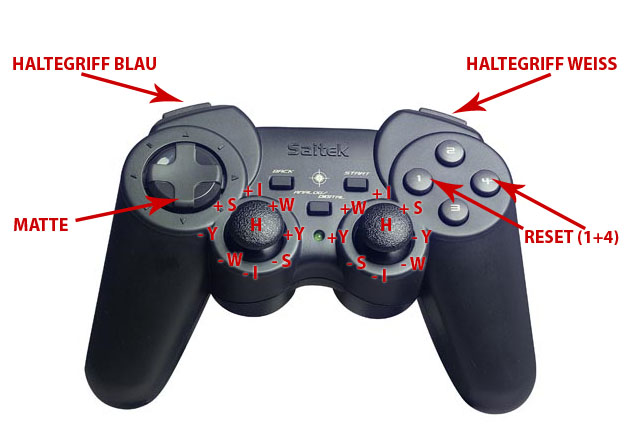
\includegraphics[width=0.8\textwidth]{images/p380.jpg}
	\caption{Übersicht Knopfbelegung}
	\label{fig:Belegung}
\end{figure}
Die Belegung der Knöpfe kann unter in den Programmeinstellungen unter dem Reiter \emph{Eingabe} geändert werden (Abb. \ref{fig:Gampad_Settings}). 
Die aktuelle Belegung ist in Abbildung \ref{fig:Belegung} bildlich dargestellt.

\mybox{{\bfseries Tipp:} Um herauszufinden, wie das jeweilige Gampad ausgerichtet ist, kann man das mitgelieferte Programm \texttt{GamepadDemo.exe} verwenden. Dort sieht man, wie die jeweiligen Achsen ausgerichtet sind und wie die Knöpfe intern nummeriert sind.}


\section{Maus-Steuerung}
Das Programm kann komplett mit der Maus gesteuert werden. Hierfür muss lediglich auf die jeweiligen Felder in der primären (eingebetteten) Anzeige oder auf die entsprechenden Knöpfe in der Oberfläche geklickt werden.

\paragraph{Punkte vergeben und zurücknehmen}
Um Punkte zu vergeben bzw. diese wieder zurückzunehmen muss lediglich in das jeweilige Feld geklickt werden. Dabei gilt Folgendes:

\begin{itemize}
	\item \emph{Punkt geben:} linke Maustaste
	\item \emph{Punkt zurücknehmen:} rechte Maustaste
\end{itemize}

\paragraph{Zeit starten/stoppen (Hajime/Matte)}
Die Kampfzeit kann mit Linksklick gestartet (gelb) und gestoppt (rot)werden.

\paragraph{Haltegriffzeit starten/stoppen (Osaekomi / Toketa)}
{Zum Starten der Haltezeit muss auf das "`00"'-Feld neben der Sanduhr geklickt werden. Der Haltegriff wird hierbei zunächst automatisch für Blau angezeigt. über das Kontextmenü dieses Feldes (Rechtsklick) kann der Haltegriff dann Weiß zugeordnet werden, falls nötig.}

Erneutes Anklicken des Feldes mit links stoppt die Haltegriffzeit.

Die Zeit wird jetzt so lange angezeigt, bis entweder erneut ein Haltegriff ausgelöst wird, oder die Hauptzeit nach Anhalten wieder läuft (=\emph{Hajime}).

\section[Besonderheiten]{Besonderheiten}
\paragraph{Sono-mama / Yoshi}
Für \emph{Sono-mama} muss man während eines Haltegriffs Matte drücken. Die Haltegriffzeit wird dann grau markiert (angehalten). Durch Drücken der jeweiligen Haltegrifftaste kann der Haltegriff wieder aufgenommen werden (\emph{Yoshi}). Zum besseren Verständnis ist der Ablauf in Abbildung \ref{fig:Ablaufdiagramm} schematisch dargestellt.
\begin{figure}[h]
	\centering
		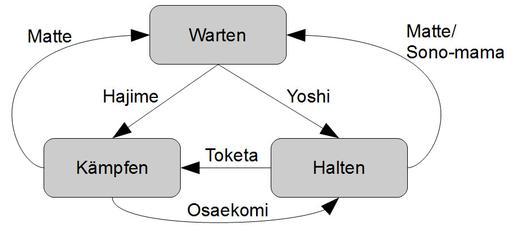
\includegraphics[width=0.8\textwidth]{images/Ablaufdiagramm.jpg}
	\caption{Ablaufdiagramm}
	\label{fig:Ablaufdiagramm}
\end{figure}

%\clearpage
\chapter{Anhang}
\section[Computer für Zweischirmbetrieb vorbereiten]{Computer für Zweischirmbetrieb vorbereiten}
\label{bkm:AnhangDualView}
Beim Anschluss des zweiten Bildschirms mit dem Computer sind folgende Punkte unbedingt zu beachten:
\begin{itemize}
	\item \textit{Desktop erweitern}
	
	Damit der zweite Bildschirm im Programm verwendet werden kann, muss er als erweiterter Desktop konfiguriert werden. Die eingestellte Auflösung spielt dabei keine Rolle, diese wird vom Programm automatisch erkannt und der Inhalt entsprechend skaliert. Falls die Darstellung auf dem Zweitmonitor nicht korrekt ist, kann sie in den Programmeinstellungen auch händisch eingestellt werden. Dies erfordert jedoch einen Neustart des Programms.

	\item \textit{Störungen abschalten}
	
	Bitte darauf achten, dass sich der Computer während der Benutzung nicht automatisch Schlafen legt (Standby) oder sich der Bildschirmschoner einschaltet. Dies kann bei neueren Computern erreicht werden, indem man diese in den Präsentationsmodus schaltet.
\end{itemize}

\end{document}
